\documentclass[]{article}

\usepackage{appendix}
\usepackage{acronym}
\usepackage{multicol}
\usepackage{graphicx}
\usepackage{rotating}

\usepackage[margin=1.25in]{geometry}


%opening
\title{Alberta E-Vent Software Overview}
\author{An Emergency Ventilator System for COVID-19}

\begin{document}
	


\maketitle

\newpage

\section*{Document History}
\begin{center}
	\begin{tabular}{ |p{3cm}| p{3cm}| p{3cm}| p{3cm}|}
		\hline
		Date & Document Status & Originator & Approver \\
		\hline 
		 \date{\today} & Draft & C. Hill \& D. Quinn &  \\  
		\hline
		 &   &  & \\ 
		 \hline
	\end{tabular}
\end{center}

\section*{Approval}

\begin{center}
	\begin{tabular}{ |p{3cm}| p{3cm}| p{3cm}| p{3cm}|}
		\hline
		Date & Name & Role & Signature \\
		\hline 
		& &  &  \\  [2ex]
		\hline
		&   &  & \\ [2ex]
		\hline 
		&   &  & \\ [2ex]
		\hline   
		&   &  & \\ [2ex]
		\hline     
	\end{tabular}
\end{center}


\clearpage

\tableofcontents

\clearpage


\section{Summary}

This report outlines the Alberta E-Vent software design, development and testing that has been undertaken.  The report is composed of four main sections:
\begin{enumerate}
	\item Functionality Overview outlining the software's high-level functionality.
	\item Process Descriptions describing the nominal operation of the ventilator modes and alarms
	\item Software Specifications outlining the full capabilities of the software.
	\item Risk Control Measures outlining the failure modes and mitigation associated with the ventilator.
	\item Verification and Validation summarizing the testing that has been conducted.
\end{enumerate}

Further summary of the performance of the ventilator to be added.

\clearpage

\section{Acronyms}

%\begin{multicols}{2}
\begin{acronym}
	
	\acro{AC}{Assist Control}
	
	\acro{BPM}{Breaths per Minute}
	
	\acro{IT}{Inspiratory Time}
	
	\acro{PEEP}{Positve End-Expiratory Pressure}
	\acro{PIP}{Peak Inspiratory Pressure}
	
	\acro{RR}{Respiratory Rate}
	
	\acro{TP}{Trigger Pressure}
	\acro{TV}{Tidal Volume}
	
	\acro{VC}{Volume Control}
	
\end{acronym}
%\end{multicols}


\clearpage

\section{Functionality Overview}

The Alberta E-Vent is a positive displacement ventilator which uses feedback control to deliver a set volume of air/oxygen to a patient.  The software supports two modes of ventilation:
\begin{itemize}
	\item Assist Control (AC) Mode
	\item Volume Control (VC) Mode
\end{itemize}
Volume Control mode is the most basic mode offered by the ventilator.  When VC mode is selected, the ventilator delivers breaths at a set rate and volume which are defined by the following properties:
\begin{enumerate}
	\item Tidal Volume - the total volume delivered to the patient during inspirations
	\item Respiratory Rate - the number of breaths delivered per minute
	\item Inspiratory Time - the duration, in seconds, over which the inhalation portion of the breath is delivered
\end{enumerate}
These three settings fully define the behavior of the ventilator. Note that the expiatory time and corresponding inhalation:exhalation (I:E) ratio are implicitly set by these three parameters and as such, neither exhale time or I:E ratio are offered as user adjustable settings.  Full details on the operation of VC Mode are given in Section \ref{sect:vcMode}.

In Assist Control (AC) Mode, the ventilator will respond to patient triggered-breaths in addition to delivering the base-line ventilation rate set by the respiratory therapist.  A patient-triggered breath occurs when the breathing circuit pressure drops by a set amount below the PEEP pressure.  This set amount is user adjustable and is referred to as the trigger pressure.  Note that the trigger pressure is always taken to be relative to the measure PEEP pressure and should not be considered an absolute pressure.  Full details on the operation of AV Mode are given in Section \ref{sect:acMode}.

\section{Software Specifications}

This section outlines the performance of the ventilator software including supported ventilation modes, user adjustable parameters, and built in system alarms and checks.  Verification and validation of these specifications are provided in Section \ref{sect:vandv}.
\subsection{Supported Modes}

The ventilator software supports the following features and specifications:
\begin{enumerate}
	\item Assist Control Mode
	\item Volume Control Mode
\end{enumerate}




\subsection{Adjustable Ventilation Parameters}


\begin{center}
	\begin{tabular}{ |p{3.8cm}| p{2.2cm}| p{2.2cm}|p{2.2cm}|}
		\hline
		\textbf{Parameter} & \textbf{Range} & \textbf{Increment}& \textbf{Default} \\
		\hline 
		Tidal Volume & 50-100\%* & 1\% & 50\% \\  
		\hline
		Respiratory Rate & 10-30 BPM  & 1 BPM & 20 BPM \\ 
		\hline   
		Inspiration Time & 0.5-3.0 s& 0.1 s & 1.5 s\\
		\hline
		Trigger Pressure** & 1-5 cm H\textsubscript{2}O & 1 cm H\textsubscript{2}O& 1 cm H\textsubscript{2}O \\
		\hline
	\end{tabular}
	
\end{center}
* Corresponds to a tidal volume range of approximately 400-800 milliliters

\noindent ** Only applies during AC Mode

\subsection{Alarms and Fault Detection}
\begin{center}
	\begin{tabular}{ |p{3.8cm}| p{2.2cm}| p{2.2cm}|p{2.2cm}|}
		\hline
		\textbf{Alarm} & \textbf{Range} & \textbf{Increment} & \textbf{Default}\\
		\hline
		High PIP & 30-70 cm H\textsubscript{2}O & 1 cm H\textsubscript{2}O & 40 cm H\textsubscript{2}O\\
		\hline
		Low PIP & 2-20 cm H\textsubscript{2}O & 1 cm H\textsubscript{2}O & 10 cm H\textsubscript{2}O\\
		\hline
		High PEEP & 15-35 cm H\textsubscript{2}O & 1 cm H\textsubscript{2}O &  20 cm H\textsubscript{2}O\\
		\hline
		Low PEEP & 0-10 cm H\textsubscript{2}O & 1 cm H\textsubscript{2}O &  3 cm H\textsubscript{2}O\\
		\hline
		High Respiratory Rate* & 15-40 BPM & 1 BPM & 35 cm H\textsubscript{2}O\\
		\hline
		Mechanical Failure & N/A & N/A & N/A\\
		\hline
		Homing Failure & N/A & N/A & N/A \\
		\hline
	\end{tabular}
	
\end{center}
* Only applies during AC Mode


\subsection{Software and Compiler Versions}
All verification and validation of the Alberta E-Vent software has been carried out using the following versions and tools:

\noindent\textbf{IDE/Compiler:} Arudino IDE version 1.8.12

\noindent\textbf{Alberta E-Vent Software:} version XXXX


\section{Process Descriptions}


\subsection{Startup and Calibration}

Upon power-up, the ventilator LCD screens will display the Albert E-Vent name and the software version for 2-seconds.  The ventilator will then proceed into a calibration procedure:
\begin{itemize}
	\item Arms will move outwards (away from the bag) until a limit switch is reached.  An audible click will be heard when the limit switch is depressed by the arms.
	\item Arms will stop momentarily and then begin to move inwards towards the edge of the bag.  They should stop just at the edge, or in slight contact, with the bag.  The ventilator will stop in this position for approximately 1-second before transitioning into ventilation.
	\item This location at the edge of the bag is referred to as the ventilator's zero point.
\end{itemize}
The full state flow diagram for the motor calibration procedure is provided in Appendix \ref{app:sfd}.


\subsection{Assist Control Mode}
\label{sect:acMode}
Assist Control Mode is characterized primarily by the ability to detect patient-triggered breaths.  When set to AC Mode, the ventilator will adhere to the following procedure:
\begin{itemize}
	\item A waiting period occurs in which the ventilator monitors the breathing circuit for a drop in pressure indicative of the patient demanding a breath.
	\item If this patient trigger is detected, or a sufficient period of time passes such that a breath is required to maintain the baseline respiratory setpoint, the ventilator delivers a breath at the set tidal volume and inspiration time.
	\item After completing the inhale, the motor arms retract to the zero point location.  This retraction period occurs over 20\% of the nominal expiration time to allow for the arms to be sufficiently positioned to deliver another breath before the end of the nominal expiration period.  Upon returning to the zero point, the ventilator cycle back to the initial waiting period. 
\end{itemize}

\subsection{Volume Control Mode}
\label{sect:vcMode}
Volume Control mode functions identically to the assist control mode except that patient triggers are not monitored for.
\begin{itemize}
	\item The ventilator delivers a breath at the set tidal volume and inspiration time.
	\item The motor arms retract to the zero point location and pause for the duration of the nominal expiration period (determined based on the inspiration time and respiratory rate).
	\item Upon pausing for the required expiration time period, the cycle restarts and the ventilator delivers another breath.
\end{itemize}

\subsection{Alarm Conditions}

Alarm conditions result in an audible (LED) and visual (piezoelectric buzzer) alert. Additionally, the alarm LCD screen displays the currently triggered alarm.  If the alarm condition is not triggered on two subsequent breaths, the alarm auto-resets and deactivates the visual, audio and LCD indicators.  The exception to this auto-reset feature are the mechanical fault and homing timeout alarms which require a motor calibration or power cycle respectively in order to reset. 

An alarm silence button mutes all active alarms for a period of 2-minutes.  If a new alarm occurs during this period the audio alert returns and any subsequent pushes of the alarm silence button will silence all active alarms for an additional two-minutes.

Additional details on the functioning of the alarms is provided by the state flow diagrams in Appendix \ref{app:sfd}.

\subsubsection{High Peak Inspiratory Pressure (PIP)}
The PIP is measured at all times when the motor arms are moving inwards to deliver a breath.  If the pressure in the breathing circuit exceeds the high PIP alarm set-point, the breath is immediately aborted. During a breath abort, the motor arms are commanded to stop and immediately move outwards to zero point at the edge of the bag.  A high PIP alarm may be triggered at any points during the inhale phase, including the plateau pressure pause that occurs at the top of the breath.  After aborting the breath, ventilation will continue with additional high PIP alarms triggering additional aborted breaths.  After two consecutive breaths that do not trigger the alarm, the alarm is auto-reset.

\subsubsection{Low Peak Inspiratory Pressure (PIP)}
The low PIP condition is checked immediately before the pause phase at the top of the breath.  This period is where the highest inspiratory pressure is found and if the measured value falls below the low PIP alarm set-point, the alarm will be triggered.  Ventilation continues as normal under this alarm but operator attention is required since a persistent low PIP alarm can be indicative of a leak or disconnection in the breathing circuit. After two consecutive breaths that do not trigger the alarm, the alarm is auto-reset.

\subsubsection{High Peak End-Expiratory Pressure (PEEP)}
The PEEP pressure is measured at either the end of the motor return period (AC Mode) or after the nominal exhalation time (VC Mode).  The measured PEEP value is then compared against the high PEEP alarm set-point.  If the measured PEEP pressure exceeds the high PEEP alarm set-point, the alarm is activated. After two consecutive breaths that do not trigger the alarm, the alarm is auto-reset.

\subsubsection{Low Peak End-Expiratory Pressure (PEEP)}
The PEEP pressure is measured at either the end of the motor return period (AC Mode) or after the nominal exhalation time (VC Mode).  The measured PEEP value is then compared against the low PEEP alarm set-point.  If the measured PEEP pressure is less than the low PEEP alarm set-point, the alarm is activated. After two consecutive breaths that do not trigger the alarm, the alarm is auto-reset.  Similar to the low PIP alarm, the low PEEP alarm can be indicative of a leak or disconnection.

\subsubsection{High Respiratory Rate (AC Mode Only)}
The respiratory rate is calculated during AC mode to account for breaths that are spontaneously triggered by the patient in addition to breaths delivered by the baseline rate set on the ventilator.  A new average respiratory rate is calculated every 5-breaths.  If the respiration rate calculated during this time exceeds the high respiratory alarm set-point, the alarm will be triggered.  If the next 5-breaths result in a calculated respiratory rate below the set-point, the alarm is auto-reset. 


\subsection{Fault Conditions}
Fault conditions require a departure from ventilation in order to correct.  There are two fault conditions that are monitored for by the software.

\subsubsection{Mechanical Failure}
A mechanical failure occurs when the commanded motor position is not reached in the allocated time.  Such a failure can occur for a number of reasons such as:
\begin{itemize}
	\item Faulty wiring
	\item Encoder failure
	\item Mechanical obstructions preventing arm motion
	\item Motor controller failure
\end{itemize}
If a mechanical failure condition is detected, ventilation is stopped and the motor attempts to re-calibrate.  If the calibration is successful, ventilation will continue.  The software keeps and internal count of the number of mechanical failures that have occurred.  In the event that two mechanical failure conditions occur, the ventilator immediately proceeds to the homing failure alarm which requires a full system restart to resolve.

\subsubsection{Homing Failure}
A homing failure alarm will occur if two mechanical failure conditions are detected during the operation of the ventilator, or if the system times out while waiting for a limit switch activation during calibration.  Either of these scenarios will activate the visual and audio components of the alarm and display a message on the LCD requiring the operator to power cycle the device.



\section{Risk Control Measures}

To be added once the risk matrix is finalized.

\section{Verification and Validation}
\label{sect:vandv}

\subsection{Servo Lung Testing}

To be completed with finalized software.


\subsubsection{Ventilation Testing}

To be completed with finalized software.


\subsubsection{Alarm Testing}

To be completed with finalized software.

\subsubsection{Clinical Feedback}

To be completed with finalized software.

\subsection{Longevity Testing}

To be completed with finalized software.



\appendix

\section{Software Flow Charts}
\label{app:sfd}

State flow diagrams summarize the behavior of the software.  Each diagram provides an overview of a particular aspect of the program.
\begin{enumerate}
	\item The overall program state flow diagram is shown in Fig. \ref{fig:main_stfd}.
	\item The motor homing and zeroing (calibration) state flow diagram is shown in Fig. \ref{fig:mz_stfd}.
	\item The Assist control Mode state flow diagram is shown in Fig. \ref{fig:ac_stfd}.
	\item The Volume Control Mode state flow diagram is shown in Fig. \ref{fig:vc_stfd}.
\end{enumerate}

Note that the combined behavior of all of these state flow diagrams is necessary for a complete understanding of how the software interacts.

\begin{figure}
	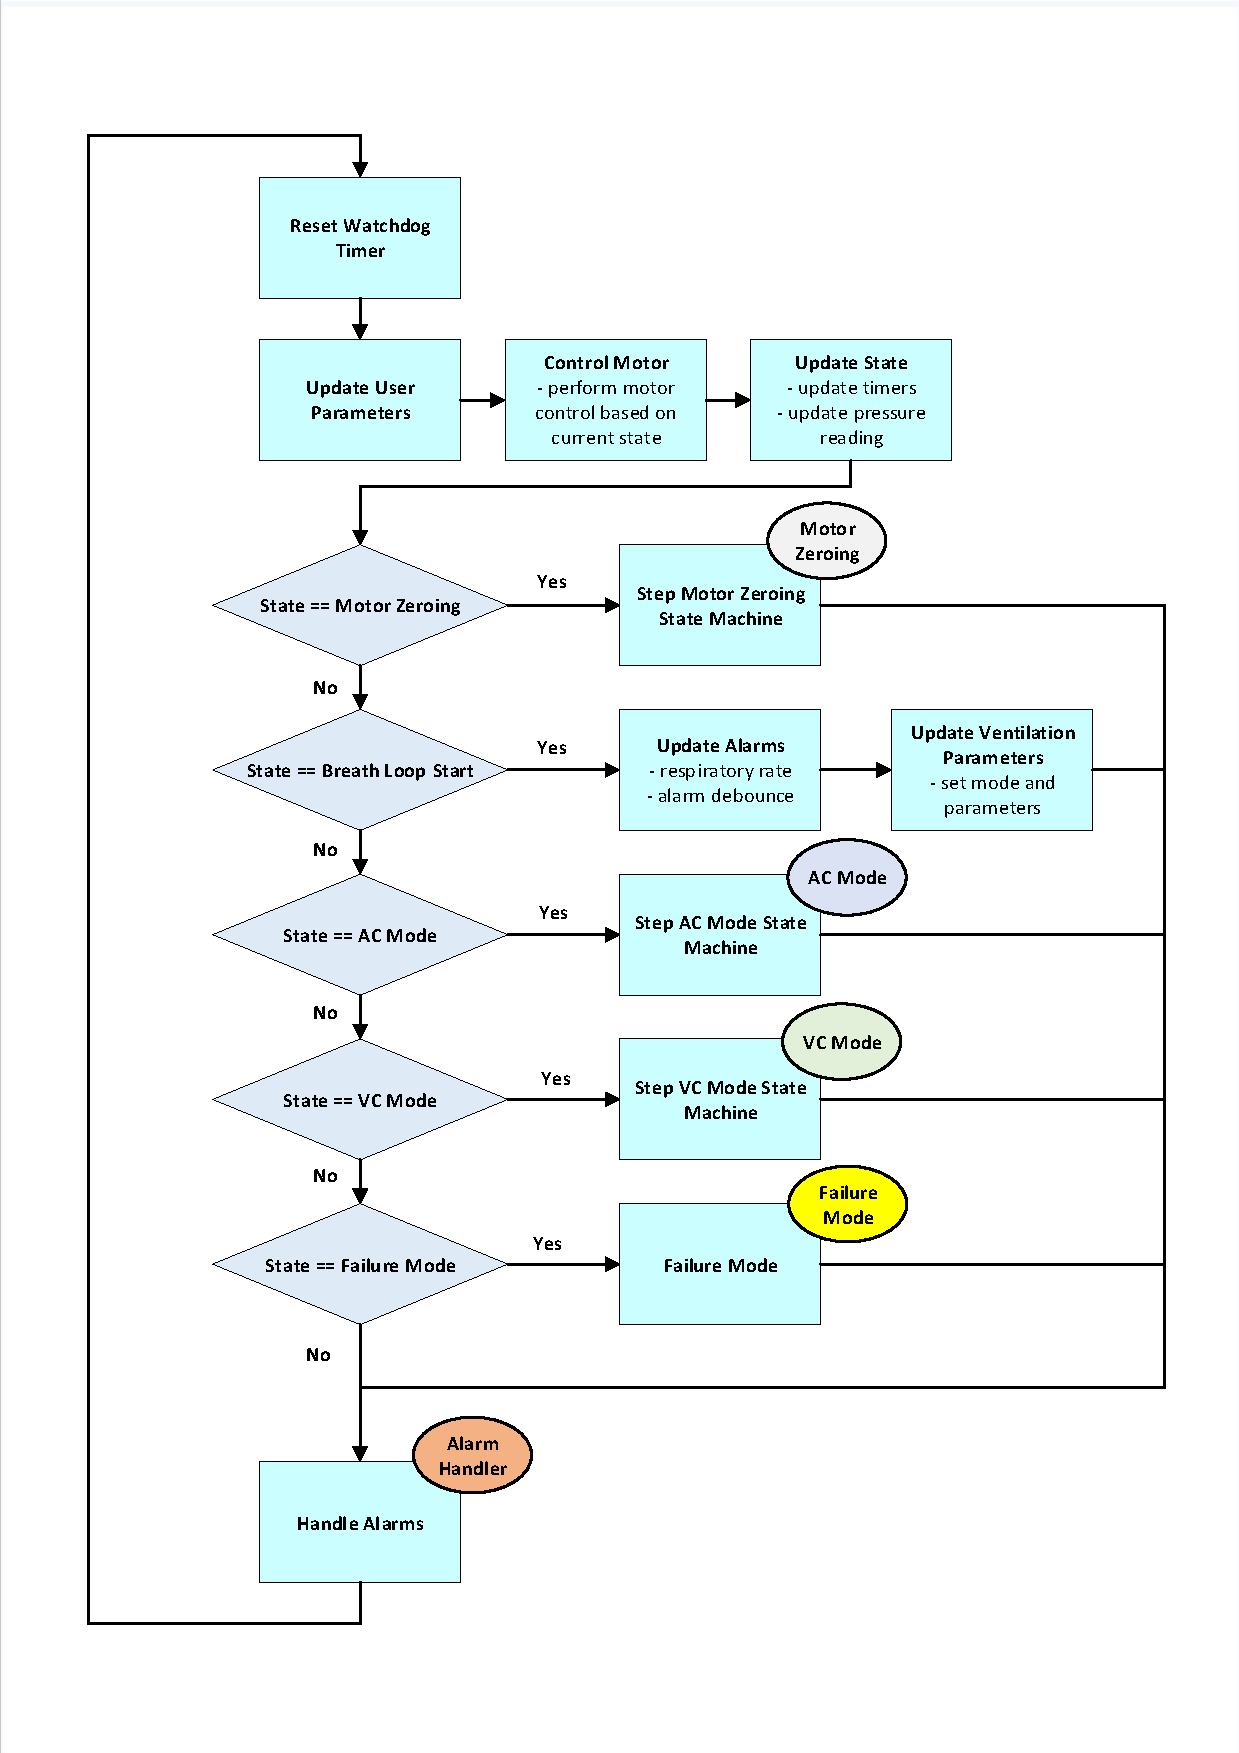
\includegraphics[scale= 0.82, trim=15 60 15 60, clip]{figures/main_loop.pdf}
	\caption{Main Program Loop}
	\label{fig:main_loop}
\end{figure}

\begin{sidewaysfigure}
	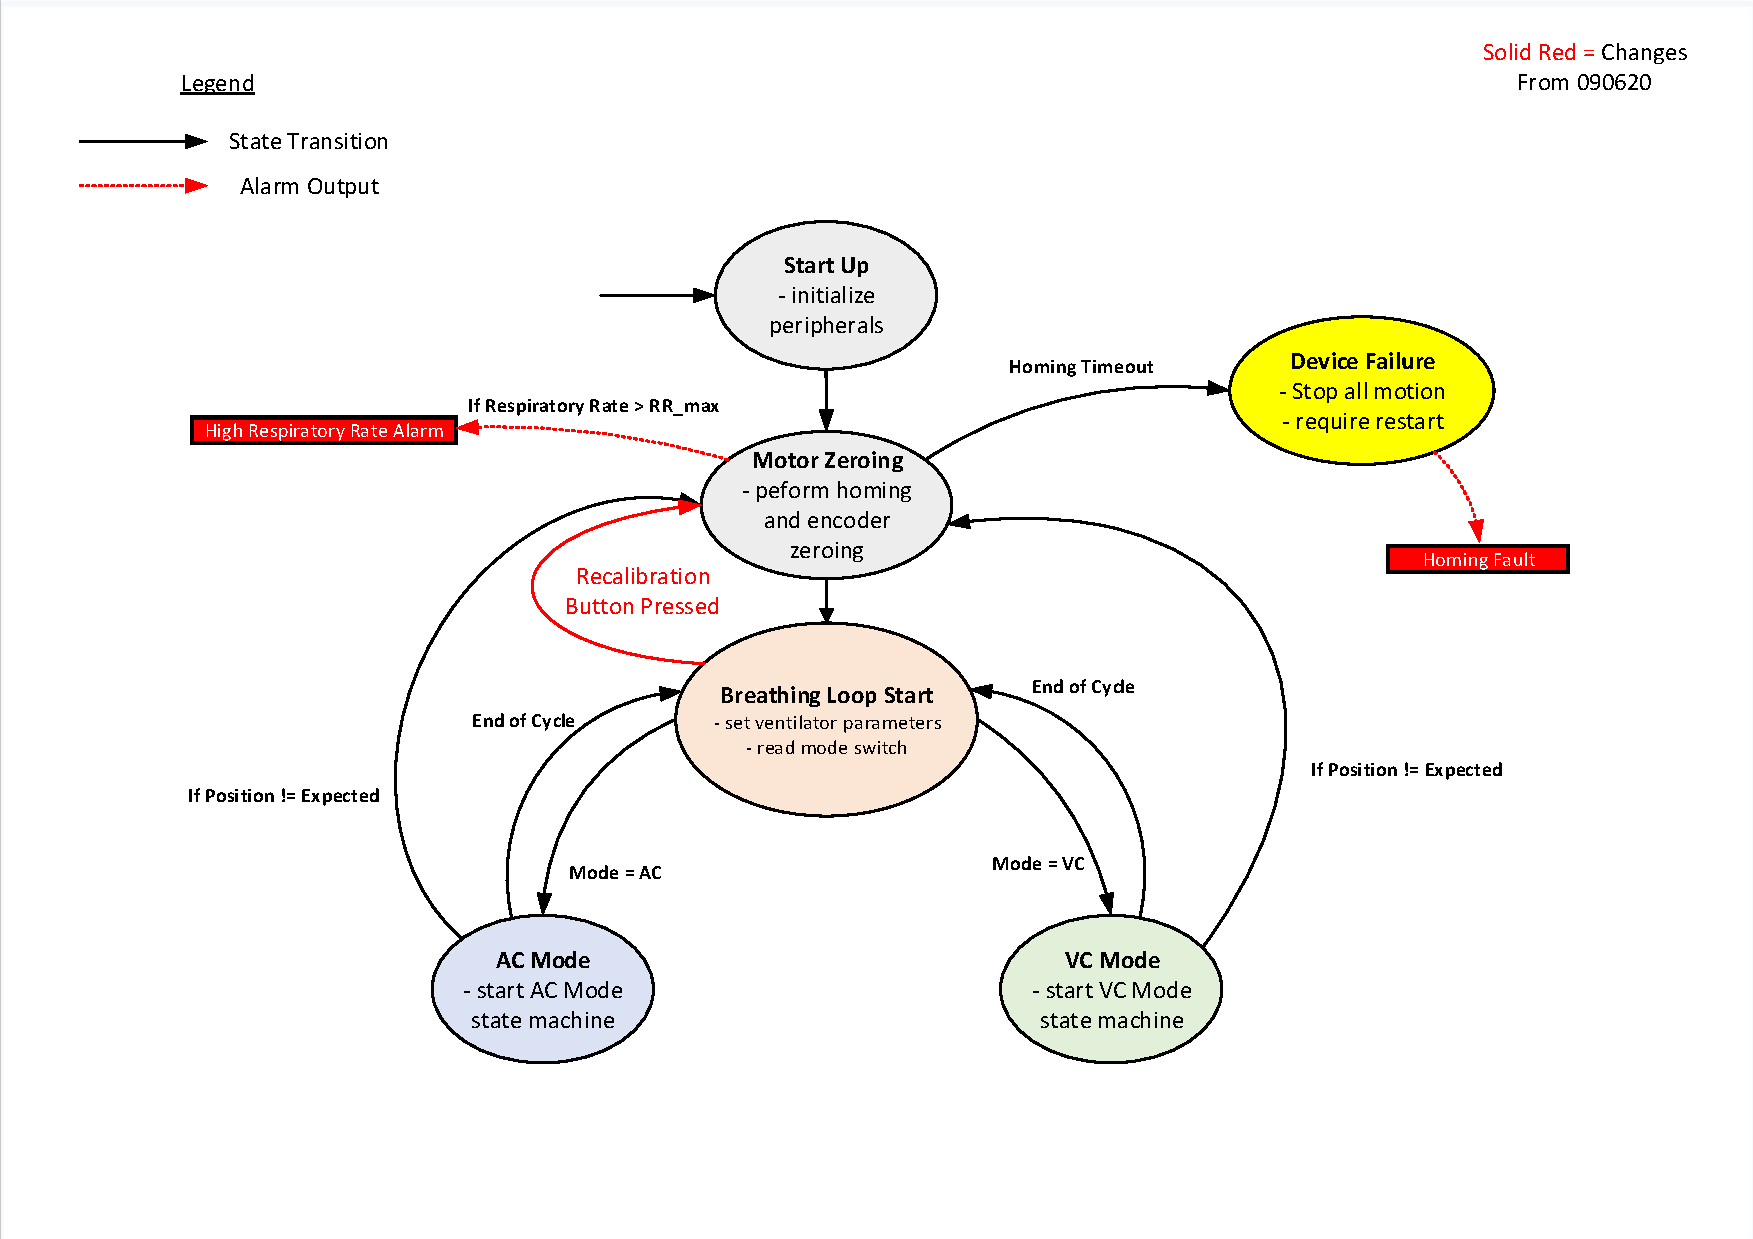
\includegraphics[scale=0.8, trim = 6 6 6 6, clip]{figures/main_state_flow.pdf}
	\caption{Overall Program State Flow Diagram}
	\label{fig:main_stfd}
\end{sidewaysfigure}

\begin{sidewaysfigure}
	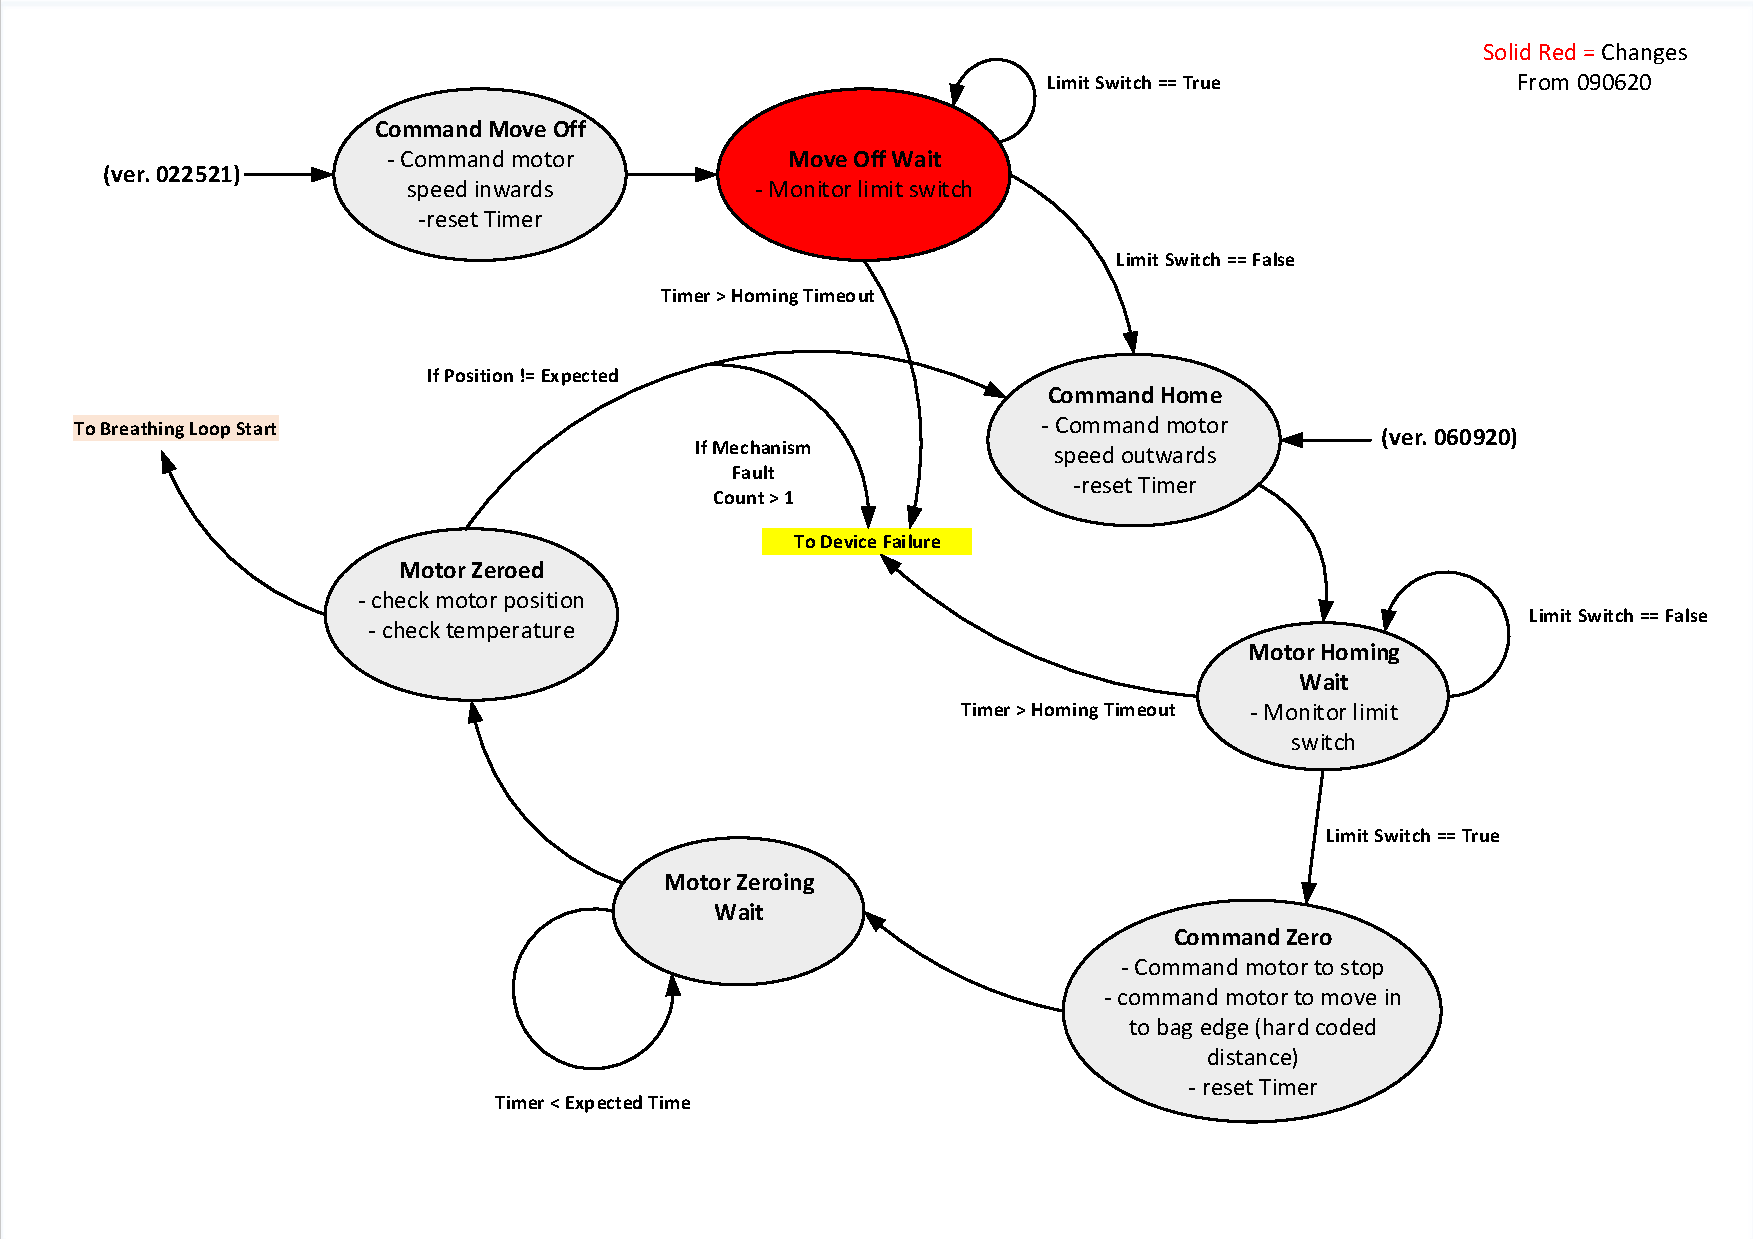
\includegraphics[scale=0.8, trim = 6 6 6 6, clip]{figures/motor_zeroing.pdf}
	\caption{Motor Zeroing State Flow Diagram}
	\label{fig:mz_stfd}
\end{sidewaysfigure}

\begin{sidewaysfigure}
	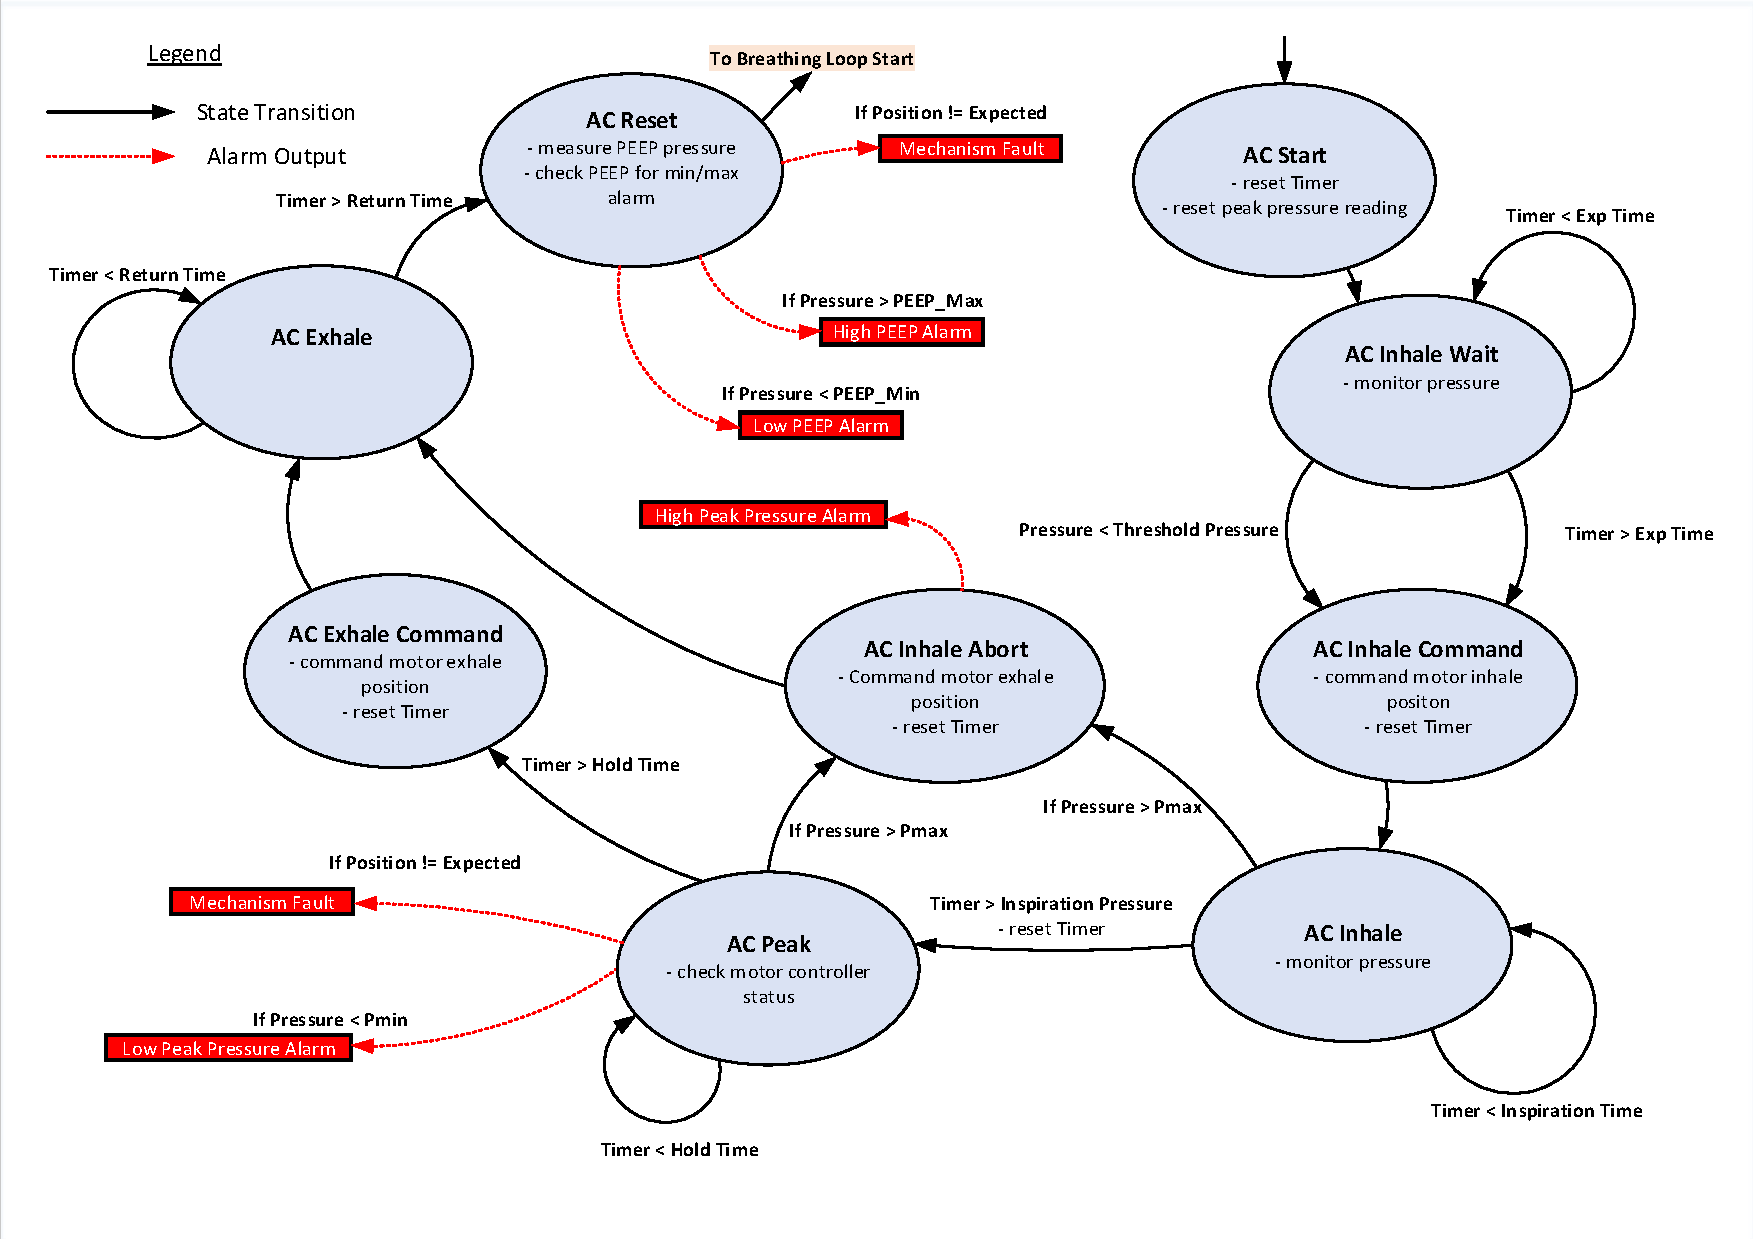
\includegraphics[scale=0.8, trim = 6 6 6 6, clip]{figures/ac_mode.pdf}
	\caption{Assist Control Mode State Flow Diagram}
	\label{fig:ac_stfd}
\end{sidewaysfigure}

\begin{sidewaysfigure}
	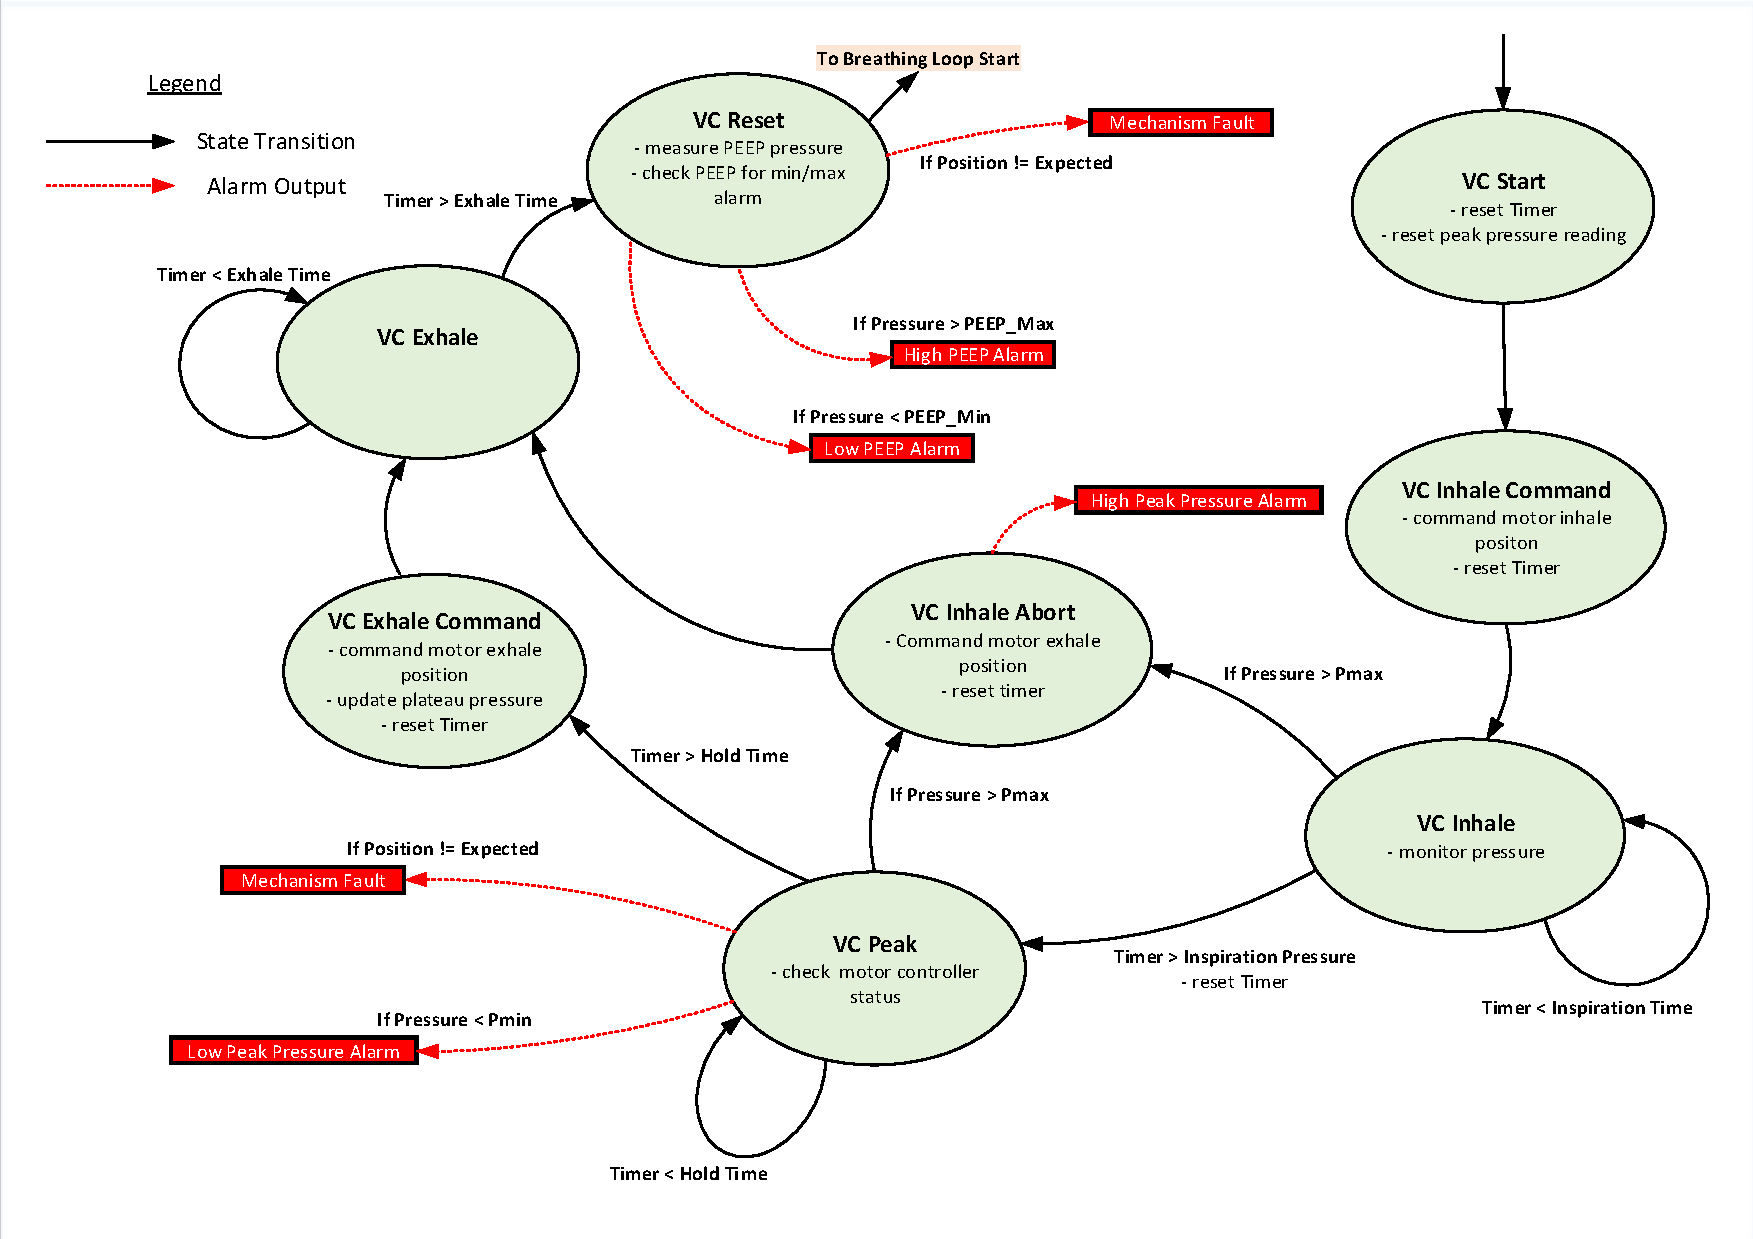
\includegraphics[scale=0.8, trim = 6 6 6 6, clip]{figures/vc_mode.pdf}
	\caption{Volume Control Mode State Flow Diagram}
	\label{fig:vc_stfd}
\end{sidewaysfigure}

\begin{figure}
	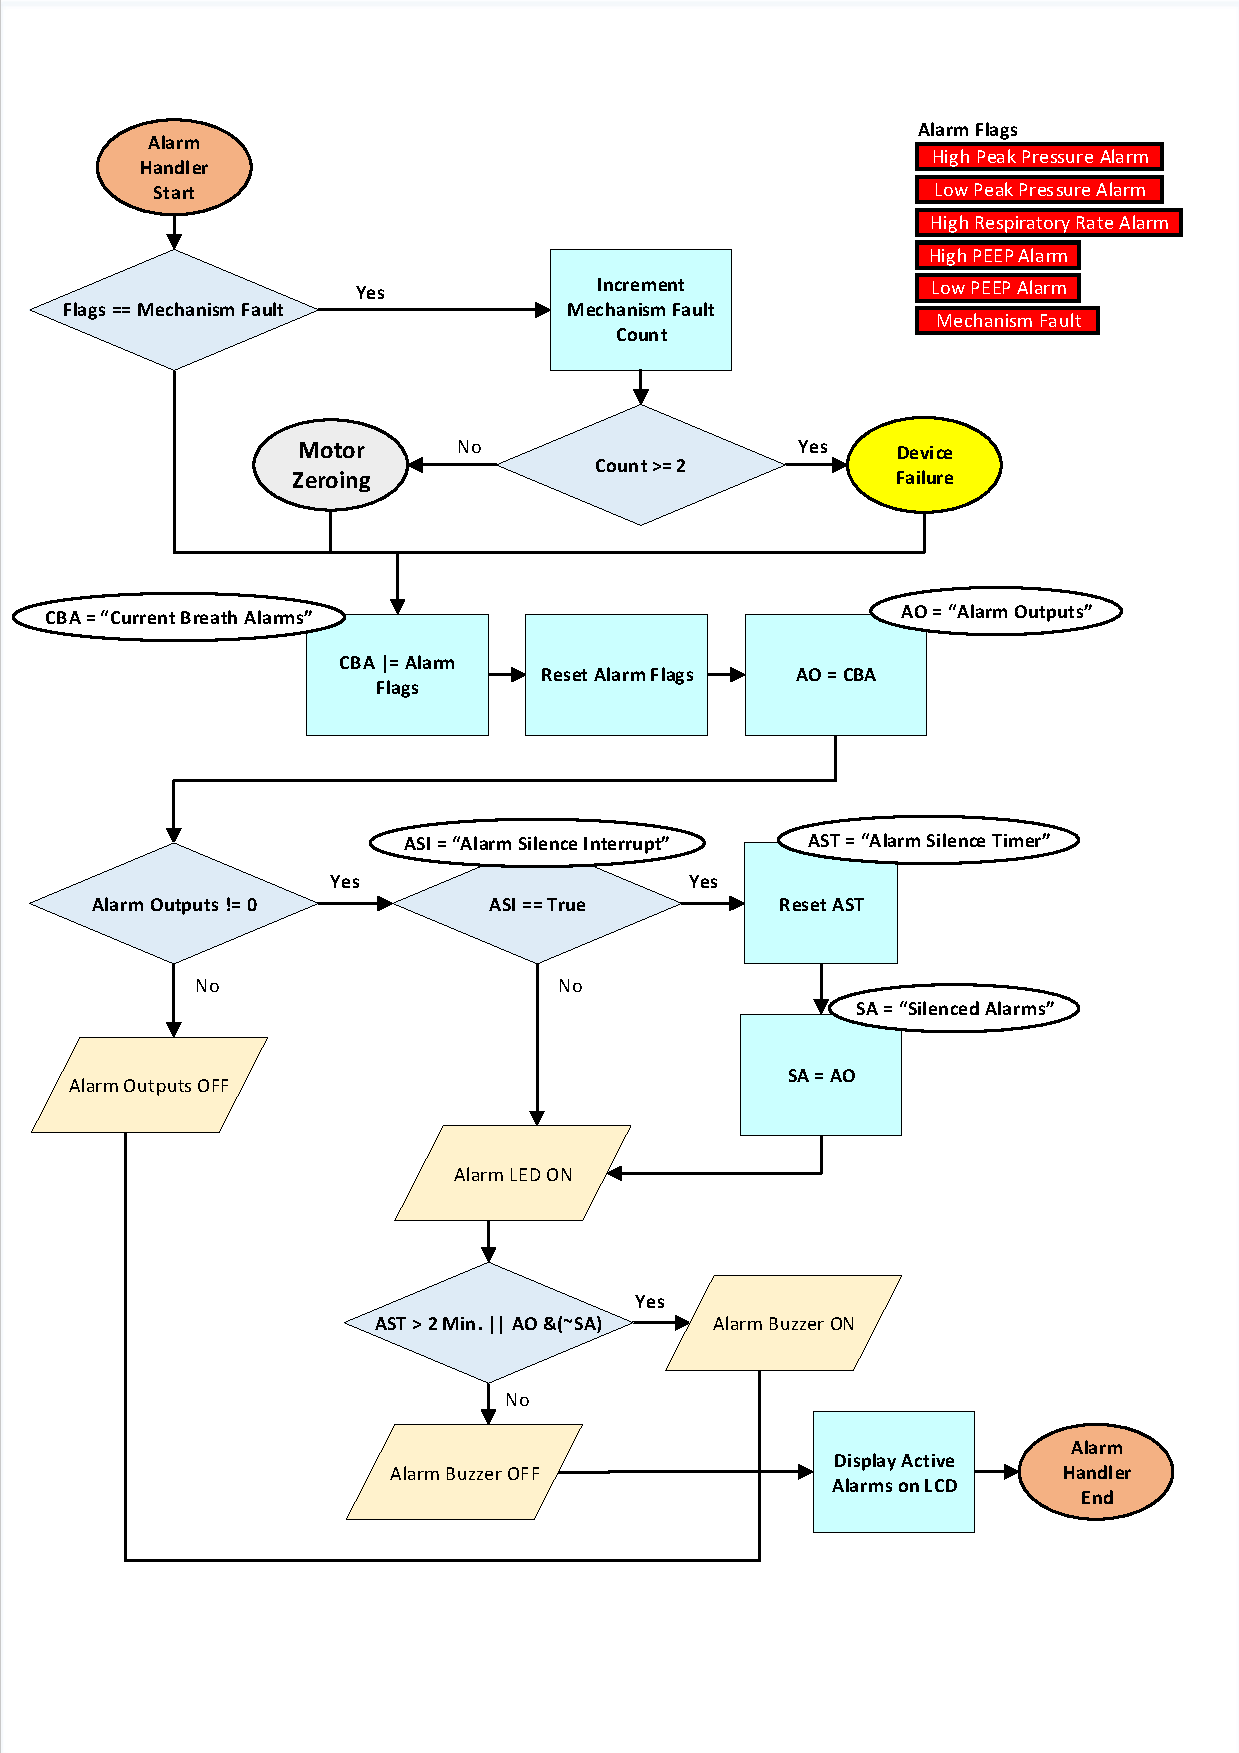
\includegraphics[scale= 0.82, trim=15 70 15 50, clip]{figures/alarm_handler.pdf}
	\caption{Alarm Handler}
	\label{fig:alarm_loop}
\end{figure}


\end{document}
